\section{多目的CAFE問題}\label{sec:background}


多目的CAFE問題は,与えられた入力から,装備および燃費に関する制約を満たしつつ,
トレードオフの関係にある複数の目的関数のもとで最適な車両装備仕様を求める問題である.
本節では,多目的CAFE問題の入力,制約,目的関数について説明し,例を用いて具体的な
入力の内容と,そこから得られる装備仕様を示す.

多目的CAFE問題の入力は以下の通りである.以降,装備タイプを{\bf タイプ},
装備オプションを{\bf オプション}と簡単に書くことにする.

\begin{enumerate} 
\setlength{\itemsep}{0cm}

 \item タイプの集合\label{input:vp}
\item オプションの集合\label{input:v}
\item タイプとオプションの対応関係\label{input:vp-v}
\item 各オプションに付加された IWR 値\label{input:iwr}
\item 各タイプで選択可能なオプション数の上下限値\label{input:ublb}
\item 必須なタイプの集合\label{input:req_vp}
\item タイプ同士,オプション同士,および,タイプとオプション間の依存関係
  \label{input:dependency}

%%%
\item 求めたい装備仕様の個数\label{input:g}
\item 各装備仕様とタイプ(あるいはオプション)間の依存関係\label{input:init}
\item CAFE 基準値\label{input:cafe}
\item 各装備仕様に含まれるオプションの IWR 値の総和と燃費との対応表\label{input:fe}
\item 各装備仕様に含まれるオプションの IWR 値の総和と予想販売台数との対応表\label{input:sv}
\end{enumerate}
入力~\ref{input:iwr}の IWR は Inertial Working Rating の略で,
直観的には各オプションの重量を表す.
入力~\ref{input:g}の個数は,求めたい派生車両の数と考えるとわかりやすい.
入力\ref{input:vp}〜\ref{input:cafe}は問題ごとに異なるが,
入力\ref{input:fe}, \ref{input:sv} は共通のものを使用する.
本論文では,これらの入力をまとめて多目的CAFE問題の{\bf 問題インスタンス}と呼ぶ.

多目的CAFE問題の制約は以下の通りである.
\begin{description}
\item[範囲制約]: 各装備仕様について,各タイプで選択されるオプション数は,
  入力~\ref{input:ublb}で与えられた上下限値の範囲内でなければならない.
\item[依存制約]: 各装備仕様について,入力~\ref{input:dependency}で与
  えられた依存関係を満たさなければならない.
  依存制約には,{\bf 要求制約}と{\bf 排他制約}の2つがある.
\item[燃費制約]: 入力~\ref{input:cafe}の CAFE 基準値を$t$,
  入力~\ref{input:g}の装備仕様個数を$n$として,
  以下の CAFE 規制を満たさなければならない.
  %\begin{adjustvboxheight}
  \[
    \begin{array}{lcr}
      & & \\
      \displaystyle\frac{\sum_{i=1}^{n} FE_{i}\cdot SV_{i}}{\sum_{i=1}^{n} SV_{i}}
      &
        \geq 
      &
        t \\
      & & 
    \end{array}
  \]
  %\end{adjustvboxheight}
  不等式の左辺は$n$個の装備仕様の\textbf{平均燃費}を表している.
  $FE_{i}$と$SV_{i}$は,装備仕様$i$の燃費と予想販売台数を表しており,
  それぞれ,入力~\ref{input:fe}と\ref{input:sv}の対応表を元に計算される.
\item[初期制約]:
  入力~\ref{input:init}で与えられた依存関係を満たさなければならない.
\end{description}

本研究では,多目的CAFE問題の目的関数として,以下の2つを用いる.
\begin{description}
 \item[予想販売台数の最大化]: 各装備仕様ごとに求められる予想販売台数の合計を最大化する.
 \item[オプション数の最小化]: 装備仕様全体で,使用されるオプションの種類の数を最小化する.
	    これは,製造ラインの削減や,大量生産を促進することを狙いとしている.
\end{description}

% %-------------------------------------------------------
% \begin{figure}[tb]
%   \centering
%   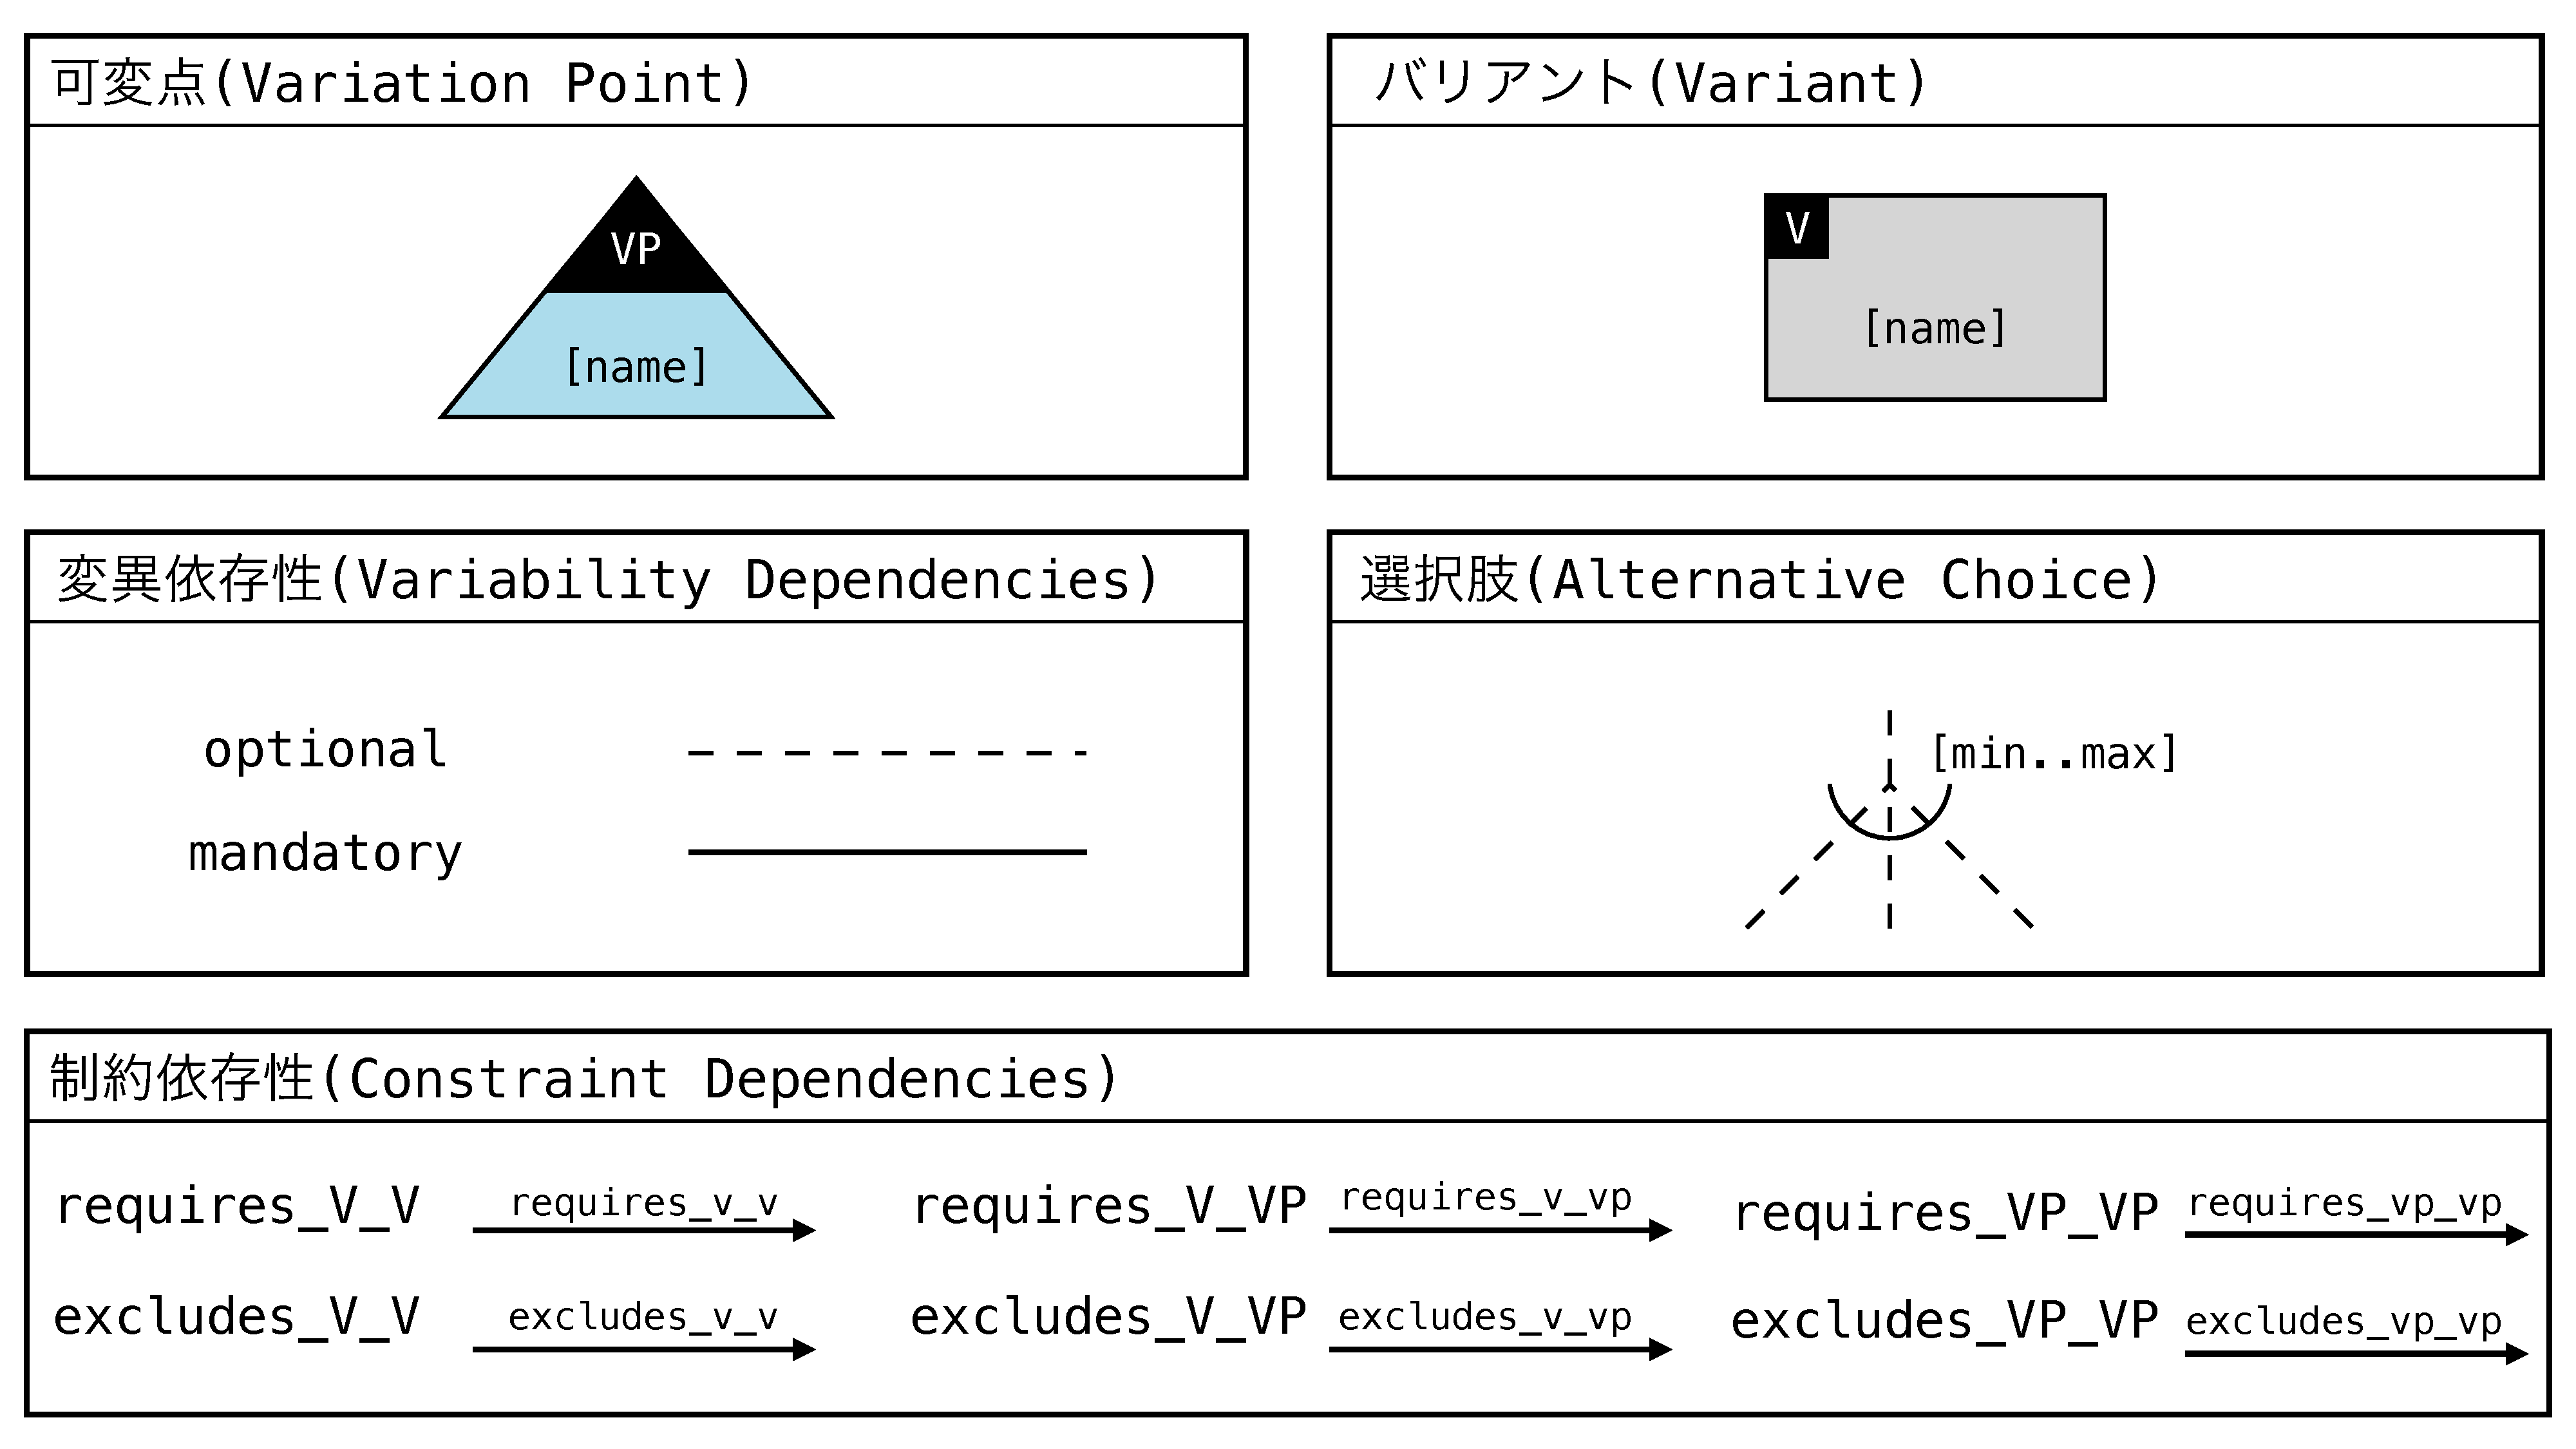
\includegraphics[width=\linewidth]{images/notation.pdf}
%   \caption{可変性モデルの表記法\cite{Pohl05:sple}}
%   \label{fig:ovm_notation}
% \end{figure}
% %-------------------------------------------------------

%-------------------------------------------------------
\begin{figure}[t]
  \centering
  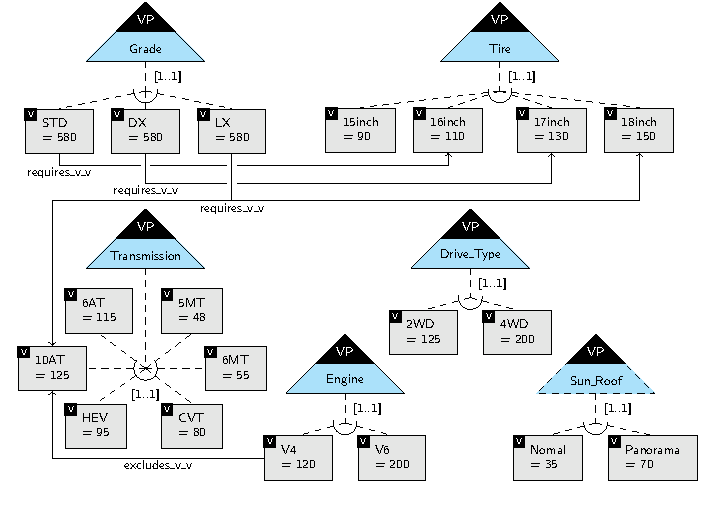
\includegraphics[width=1.1\linewidth]{images/ovm_example.pdf}
  \caption{CAFE問題の例}
  \label{fig:ovm_example}
\end{figure}
%-------------------------------------------------------

多目的CAFE問題の例を図~\ref{fig:ovm_example}に示す.
この例は,ソフトウェアプロダクトライン開発の分野で用いられる
\textbf{可変性モデル} (Orthogonal Variability Model; OVM\cite{Pohl05:sple})
によって記述されている.
{\sf VP}とタグ付けされている三角形のノードはタイプを,{\sf V}とタグ付けされている
四角形のノードはオプションとそのIWR値を表しており,入力\ref{input:vp}, 
\ref{input:v}, \ref{input:iwr}に相当する.
対応関係にあるタイプとオプションは点線で結ばれており(入力\ref{input:vp-v}),
付記される$[1..1]$のような多重度は入力\ref{input:ublb}の各タイプで選択可能な
オプション数の上下限値を意味する.
タイプ同士,オプション同士,および,タイプとオプション間を結ぶ矢印は
入力\ref{input:dependency}の依存関係を表し,要求(requires)と
排他(excludes)の2種類がある.

図~\ref{fig:ovm_example}の問題例は,
6個のタイプ,19個のオプション,5個の依存制約から構成され,
各タイプの選択可能なオプション数はすべて1である.
本論文では,実線のノードで表すタイプは,各装備仕様に対して必須とし,
\textsf{Sun\_Roof}のような選択可能なタイプ(必須ではないタイプ)
については,破線のノードで表すものとする.


% 図~\ref{fig:ovm_notation}に,可変性モデルの基本的な表記法を示す.
% 可変性モデルでは,
% 仕様ごとに変わりうる項目を\textbf{可変点}と呼び,三角形で表す.
% 可変点の具体的なインスタンスを\textbf{バリアント}と呼び,長方形で表す.
% 可変点とバリアントの対応関係には\textbf{変異依存性}と\textbf{選択肢}があり,
% 選択肢の場合は,その多重度も付記される.
% 可変点同士,バリアント同士,および,可変点とバリアント間の依存関係は,
% \textbf{制約依存性}によって表される.
% 制約依存性には,要求(\textsf{requires})と排除(\textsf{excludes})の2種類がある.

% 可変性モデルでCAFE問題を記述する場合,
% タイプは可変点,
% オプションとその IWR 値はバリアント,
% タイプとオプションの対応関係および
% 選択可能なオプション数の上下限値は選択肢,
% タイプ同士,オプション同士,および,タイプとオプション間の依存関係は
% 制約依存性によって表される.
% 以上から,CAFE問題の入力のうち,
% \ref{input:vp}〜\ref{input:iwr}は可変性モデルによって記述されるこ
% とがわかる.

% 図~\ref{fig:ovm_example}の問題例は,
% 6個のタイプ,19個のオプション,5個の依存制約から構成され,
% 各タイプの選択可能なオプション数はすべて1である.
% 本論文では,可変点で表されるタイプは,各装備仕様に対して必須とする.
% ただし,\textsf{Sun\_Roof}のような選択可能なタイプ(必須ではないタイプ)
% については,破線の可変点で表すものとする.

%-------------------------------------------------------
\begin{table}[t]
  \centering
  \caption{多目的CAFE問題(図~\ref{fig:ovm_example})の解}
  \begin{tabular}{l|l|c|c|c} \hline
    %\multicolumn{1}{c|}{装備}   & \multicolumn{3}{c}{装備仕様} \\ \cline{2-4}
    \multicolumn{2}{l|}{装備仕様}               & 1	& 2 	 & 3	\\  \hline
    装備 & \textsf{Grade}        & \textsf{STD}    & \textsf{DX}     & \textsf{LX}\\
    &\textsf{Drive\_Type}  & \textsf{2WD}    & \textsf{2WD}    & \textsf{4WD}\\
    &\textsf{Engine}	  & \textsf{V6}     & \textsf{V6}     & \textsf{V6}\\
    &\textsf{Tire}	  & \textsf{16inch} & \textsf{17inch} & \textsf{18inch}\\
    &\textsf{Transmission} & \textsf{6AT}    & \textsf{HEV}    & \textsf{10AT}\\
    &\textsf{Sun\_Roof}    & -               & -              & -  \\ \hline
    \multicolumn{2}{l|}{IWR 値の総和}           & 1,130  & 1,130   & 1,255 \\ %\hline
    \multicolumn{2}{l|}{燃費(km/L)}      & 8.8  & 8.8     & 8.0 \\ %\hline
    \multicolumn{2}{l|}{予想販売台数}    & 2,007   & 2,007   & 1,511  \\ \hline
    \multicolumn{2}{l|}{平均燃費(km/L)}  & \multicolumn{3}{c}{8.5} \\ 
    \multicolumn{2}{l|}{予想販売台数(合計)}  & \multicolumn{3}{c}{5,525} \\ 
    \multicolumn{2}{l|}{オプション数} & \multicolumn{3}{c}{12}	\\ \hline
 \end{tabular}
 \label{tab:ovm_ans}
\end{table}
%-------------------------------------------------------

図~\ref{fig:ovm_example}の問題に対する解の例を表\ref{tab:ovm_ans}に示す.
この解は,
CAFE 基準値に8.5km/L,
求めたい装備仕様の個数に3を与え,
装備仕様とオプションの依存関係として,
(装備仕様1, \textsf{STD}),
(装備仕様2, \textsf{DX}),
(装備仕様3, \textsf{LX})
を要求して得られたものである.
各装備仕様の燃費は,左から順に 8.8, 8.8, 8.0km/L と
個々には CAFE 基準値を満たしていないものもあるが,
3台の平均燃費は 8.581km/L となり,CAFE 規制を満たしている.
